%%%%%%%%%%%%%%%%%%%%%%%%%%%%%%%%%%%%%%%%%%%%%%%%%%%%%%%%%%%%%%%%%%%%%%%%%%%%%
%
% This is a LaTeX file for an A3 poster.
%
%%%%%%%%%%%%%%%%%%%%%%%%%%%%%%%%%%%%%%%%%%%%%%%%%%%%%%%%%%%%%%%%%%%%%%%%%%%%%

%%%%%%%%%%%%%%%%%%%%%%%%%%%%%%%%%%%%%%%%%%%%%%%%%%%%%%%%%%%%%%%%%%%%%%%%%%%%%
%%%%%%%%%%%%%%%%%%%%%%%%%%%%%%%%%%%%%%%%%%%%%%%%%%%%%%%%%%%%%%%%%%%%%%%%%%%%%
%
% Asymptotic behavior of solutions to the generalized Becker-Döring
% equations for general initial data.
%
% Poster for the HYKE-3 meeting in Rome, 13-15 April 2005.
%
%%%%%%%%%%%%%%%%%%%%%%%%%%%%%%%%%%%%%%%%%%%%%%%%%%%%%%%%%%%%%%%%%%%%%%%%%%%%%
%%%%%%%%%%%%%%%%%%%%%%%%%%%%%%%%%%%%%%%%%%%%%%%%%%%%%%%%%%%%%%%%%%%%%%%%%%%%%

\documentclass[american]{article}
% To modify the size of the page:
\usepackage[dvips,paperwidth=34in,paperheight=44in,landscape,centering,left=3.0cm,right=3.0cm,top=3.0cm, bottom=3.0cm]{geometry}
\usepackage{babel}
\usepackage{multicol}
\usepackage[utf8]{inputenc}
\usepackage{color,xcolor}
\usepackage{float}
\usepackage{amsmath, amsthm, amsfonts}
\usepackage{graphicx}           % Include figure files.
\usepackage{anyfontsize}
\usepackage{setspace}
\usepackage{lipsum}
% Colors
% -------
\usepackage[immediate]{silence}
\WarningFilter[temp]{latex}{Command} % silence the warning
\definecolor{azulcielo}{RGB}{227,243,248}

\newcommand\Mark[1]{\textsuperscript#1}
\pagestyle{empty}

\def\to{\rightarrow}
\usepackage{geometry}
\usepackage{layout}
\usepackage{url}
\usepackage[pdftex, pdfborderstyle={/S/U/W 0}]{hyperref}
\usepackage{csquotes}
\usepackage[backend=biber, style=ieee,language=auto]{biblatex}
\addbibresource{bibliography.bib}

\graphicspath{{media/images/}}
\DeclareGraphicsExtensions{.jpeg,.png,.jpg}
\usepackage{sectsty}
\sffamily
\sectionfont{\fontsize{60}{72}\selectfont}
%\renewcommand{\familydefault}{\sfdefault}
\usepackage{libertine}
%\usepackage{newtxtext}
%\usepackage{libertinust1math}
\usepackage{newtxmath}
\usepackage[T1]{fontenc}

\newcommand\pd[2]{\frac{\partial #1}{\partial #2}}
\newcommand\inte{\int_{\Omega^e}}
\newcommand\pinte{\int_{\partial\Omega^e}}
\newcommand\ve[1]{\mathbf{#1}}
% ===========================================================================
\usepackage{array}
\title{}
\author{}
\date{}

\begin{document}
%\maketitle

\begin{center}
  \begin{minipage}{.16\linewidth}
  \qquad\qquad
    
\includegraphics[width=\linewidth]{media/images/oden-logo-2019.png}
    ~\vfill
    ~\vfill
  \end{minipage}
  %&
  %\vspace{-0.75cm}
  \begin{minipage}{.6\linewidth}
    \begin{center}
       \textsf{\textbf{{\fontsize{90}{108}\selectfont  Developing a Compound Flooding Model using the Discontinuous Galerkin Method}}}\\\vspace{1cm}
       \textrm{\fontsize{40}{48}\selectfont Chayanon (Namo) Wichitrnithed\Mark{1}, Eirik Valseth\Mark{1}, Clint Dawson\Mark{1} \\\vspace{5mm} \Mark{1}\textit{The Oden Institute for Computational Engineering and Sciences at the University of Texas at Austin} \vspace{5mm} }
    \end{center}
  \end{minipage}
  %&
  \hspace{.03\linewidth}
    \begin{minipage}{.16\linewidth}
  \qquad\qquad
    
\includegraphics[width=\linewidth]{media/images/msi_logo.png}
    ~\vfill
    ~\vfill
  \end{minipage}
\end{center}

%\vspace{0.5cm}

\hrulefill
\vspace{10mm}
% ---------------------------------------------------------------------------
\fontsize{30}{36}\selectfont
\setlength{\columnsep}{1cm}
\vspace{-1.00cm}
\begin{multicols}{3}
% ---------------------------------------------------------------------------
% En caso de no poner resumen se comenta la siguiente sección
% ---------------------------------------------------------------------------
\noindent

\section*{Introduction}

\begin{center}
  \vspace{5mm}
  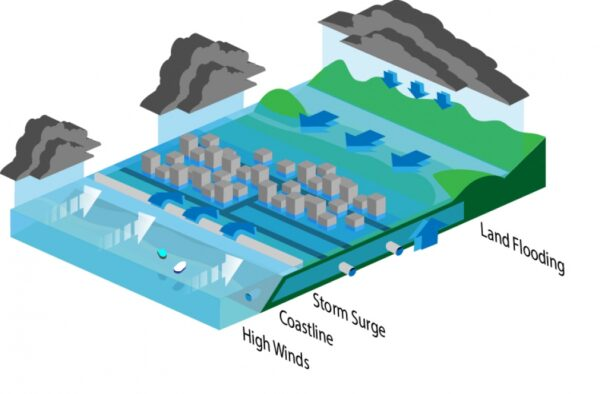
\includegraphics[width=0.95\linewidth]{media/compound.jpg}
  Figure 1: Components of compound flooding
\end{center}

\noindent Compound flooding is a complex phenomena that arises when storm surge occurs simultanteously with rainfall and river discharge. The combined effect of these components are devastating, as seen in Hurricane Harvey in 2017, where [...] occur together. The combined nature of compound flooding also makes it difficult to simulate because the model has to be able to account for these different sources and handle their numerical effects.

Regular storm surge and flooding simulations are usually run on the Advanced Circulation Model (ADCIRC), a computer program that discretizes the fluid on a 2D finite element mesh. This works fine with normal types of storm surges and flooding, but it is difficult to add source terms that account for parts of compound flooding, in this case rainfall. Moreover, the continuous Galerkin method (CG) used in ADCIRC does not guarantee mass conservation in each element which can lead to inaccuracies when source terms are added.
Due to these limitations, we incorporate rainfall into the Discontinuous Galerkin Shallow Water Equation model (DGSWEM), another model based on ADCIRC but uses the discontinuous Galerkin method (DG). In what follows, we show details of the implementation and its advantage over the regular CG method.

\section*{Model}
In ADCIRC, the continuity equation is modeled using the GWCE, which is complicated. In DG we instead use the shallow water equations (SWE), which approximate a thin layer of water in two dimensions. The continuity equation in this case is simply
\begin{align*}
  \pd{\zeta}{t} + \pd{}{x} (Hu) + \pd{}{y} (Hv) = \color{red} S(t,x,y)
\end{align*}
where $\zeta$ is the water elevation, $H$ is the total height of the water column, $u$ and $v$ the veloocities in $x$ and $y$ directions, and $\color{red} S$ is the rainfall measured in inch per second per unit area. Rainfall can vary among different parts of the domain, but here we use a constant rainfall.

\begin{center}
  \vspace{5mm}
  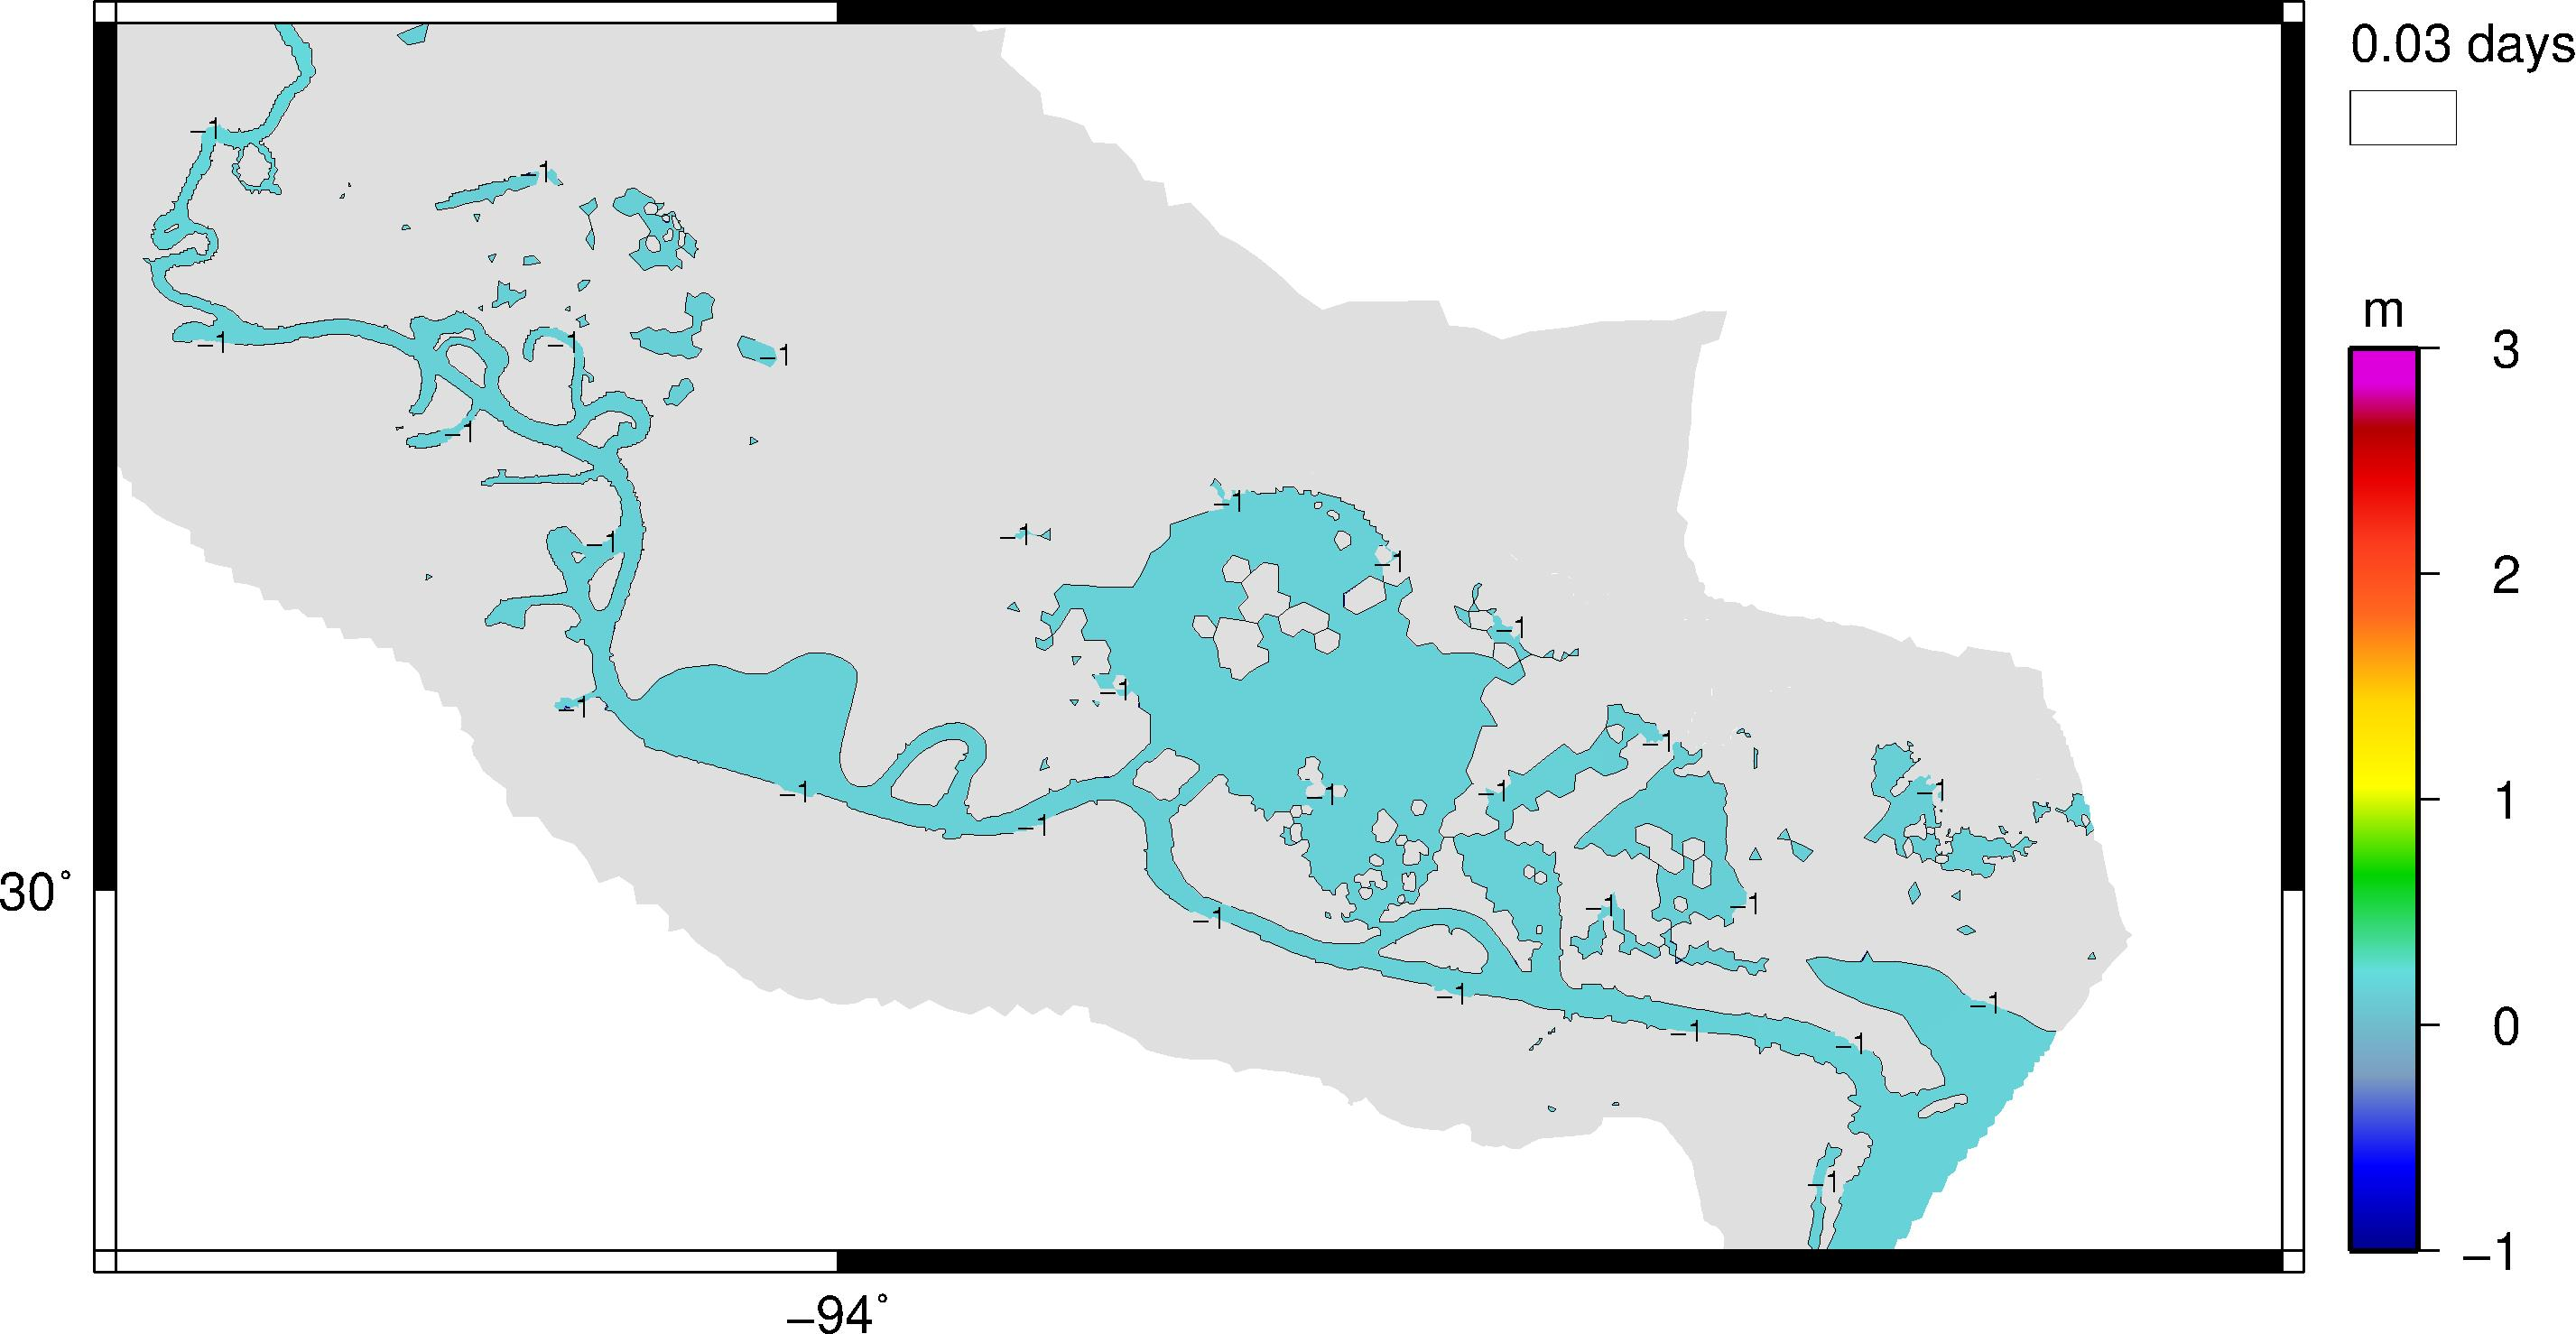
\includegraphics[width=0.95\linewidth]{media/grid.jpg}
  Figure 1: Finite element mesh of the Neches river
\end{center}

The test case is the Neches river domain in Figure 1, triangulated to around 60,000 nodes. We model the flow in which river discharge from Hurricane Harvey comes from the top left.
\section*{Method}
The DG method differs from CG in that it enforces the weak formulation on each individual element, and the solutions are allowed to be discontinuous across elements. Since the governing equations are based on conservation laws, this guarantees that water elevation is conserved in each element, aside from inflow and outflow. In mathematical terms, we have
\begin{align*}
  \inte \pd{\zeta^h}{t} v - \inte \nabla v \cdot \ve{F_1} + \pinte v \ve{\widehat{F}_1} \cdot \ve{n}  = \inte v S
\end{align*}
as the weak formulation for the continuity equation. Here, $F_1$ is the vector $[uH, vH]^T$, $v$ is the test function on $\Omega^e$, and $\ve{\widehat{F}_1}$ is the appropriate numerical flux (here we use the Roe flux).
\begin{center}
  \vspace{5mm}
    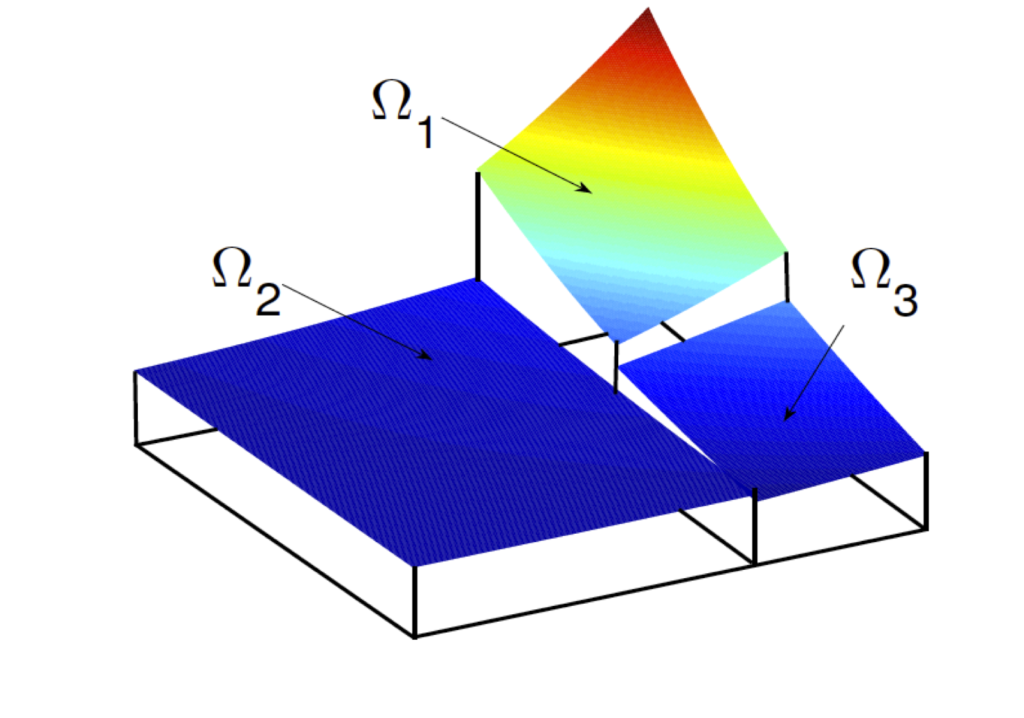
\includegraphics[width=0.55 \linewidth]{media/dg.png} \\
    Figure 2: A DG mesh with quadrilateral elements
\end{center}

Solving this system yields a system of ODEs which we then solve using a second order Strong Stability Preserving Runge-Kutta scheme (SSPRK)
\begin{align*}
  \ve{w}_h^{(1)} = \ve{w}_h^{(t)}
\end{align*}
The solution $w^h$ at the nodes is the average value of each discontinuous solution from the neighboring elements.

We account for river discharge from Hurricane Harvey (top left of the domain) by supplying the rates of flow $u$ and $v$ on element boundaries through the numerical flux.

The code is parallelized using MPI.

\section*{Results}
We ran DGSWEM on the Neches domain with 1 inch of rain per hour, constant throughout the whole domain. The simulation was run with 128 CPU cores at a time step of 0.1 seconds for 6 simulation days, which took around 8 hours in real time. The elevation plot after 6 days is given in Figure 3. As can be seen, the flow is compounded by the river discharge from the top left corner as well as rainfall on the other part of the domain.
\begin{center}
    \vspace{0.5cm}
    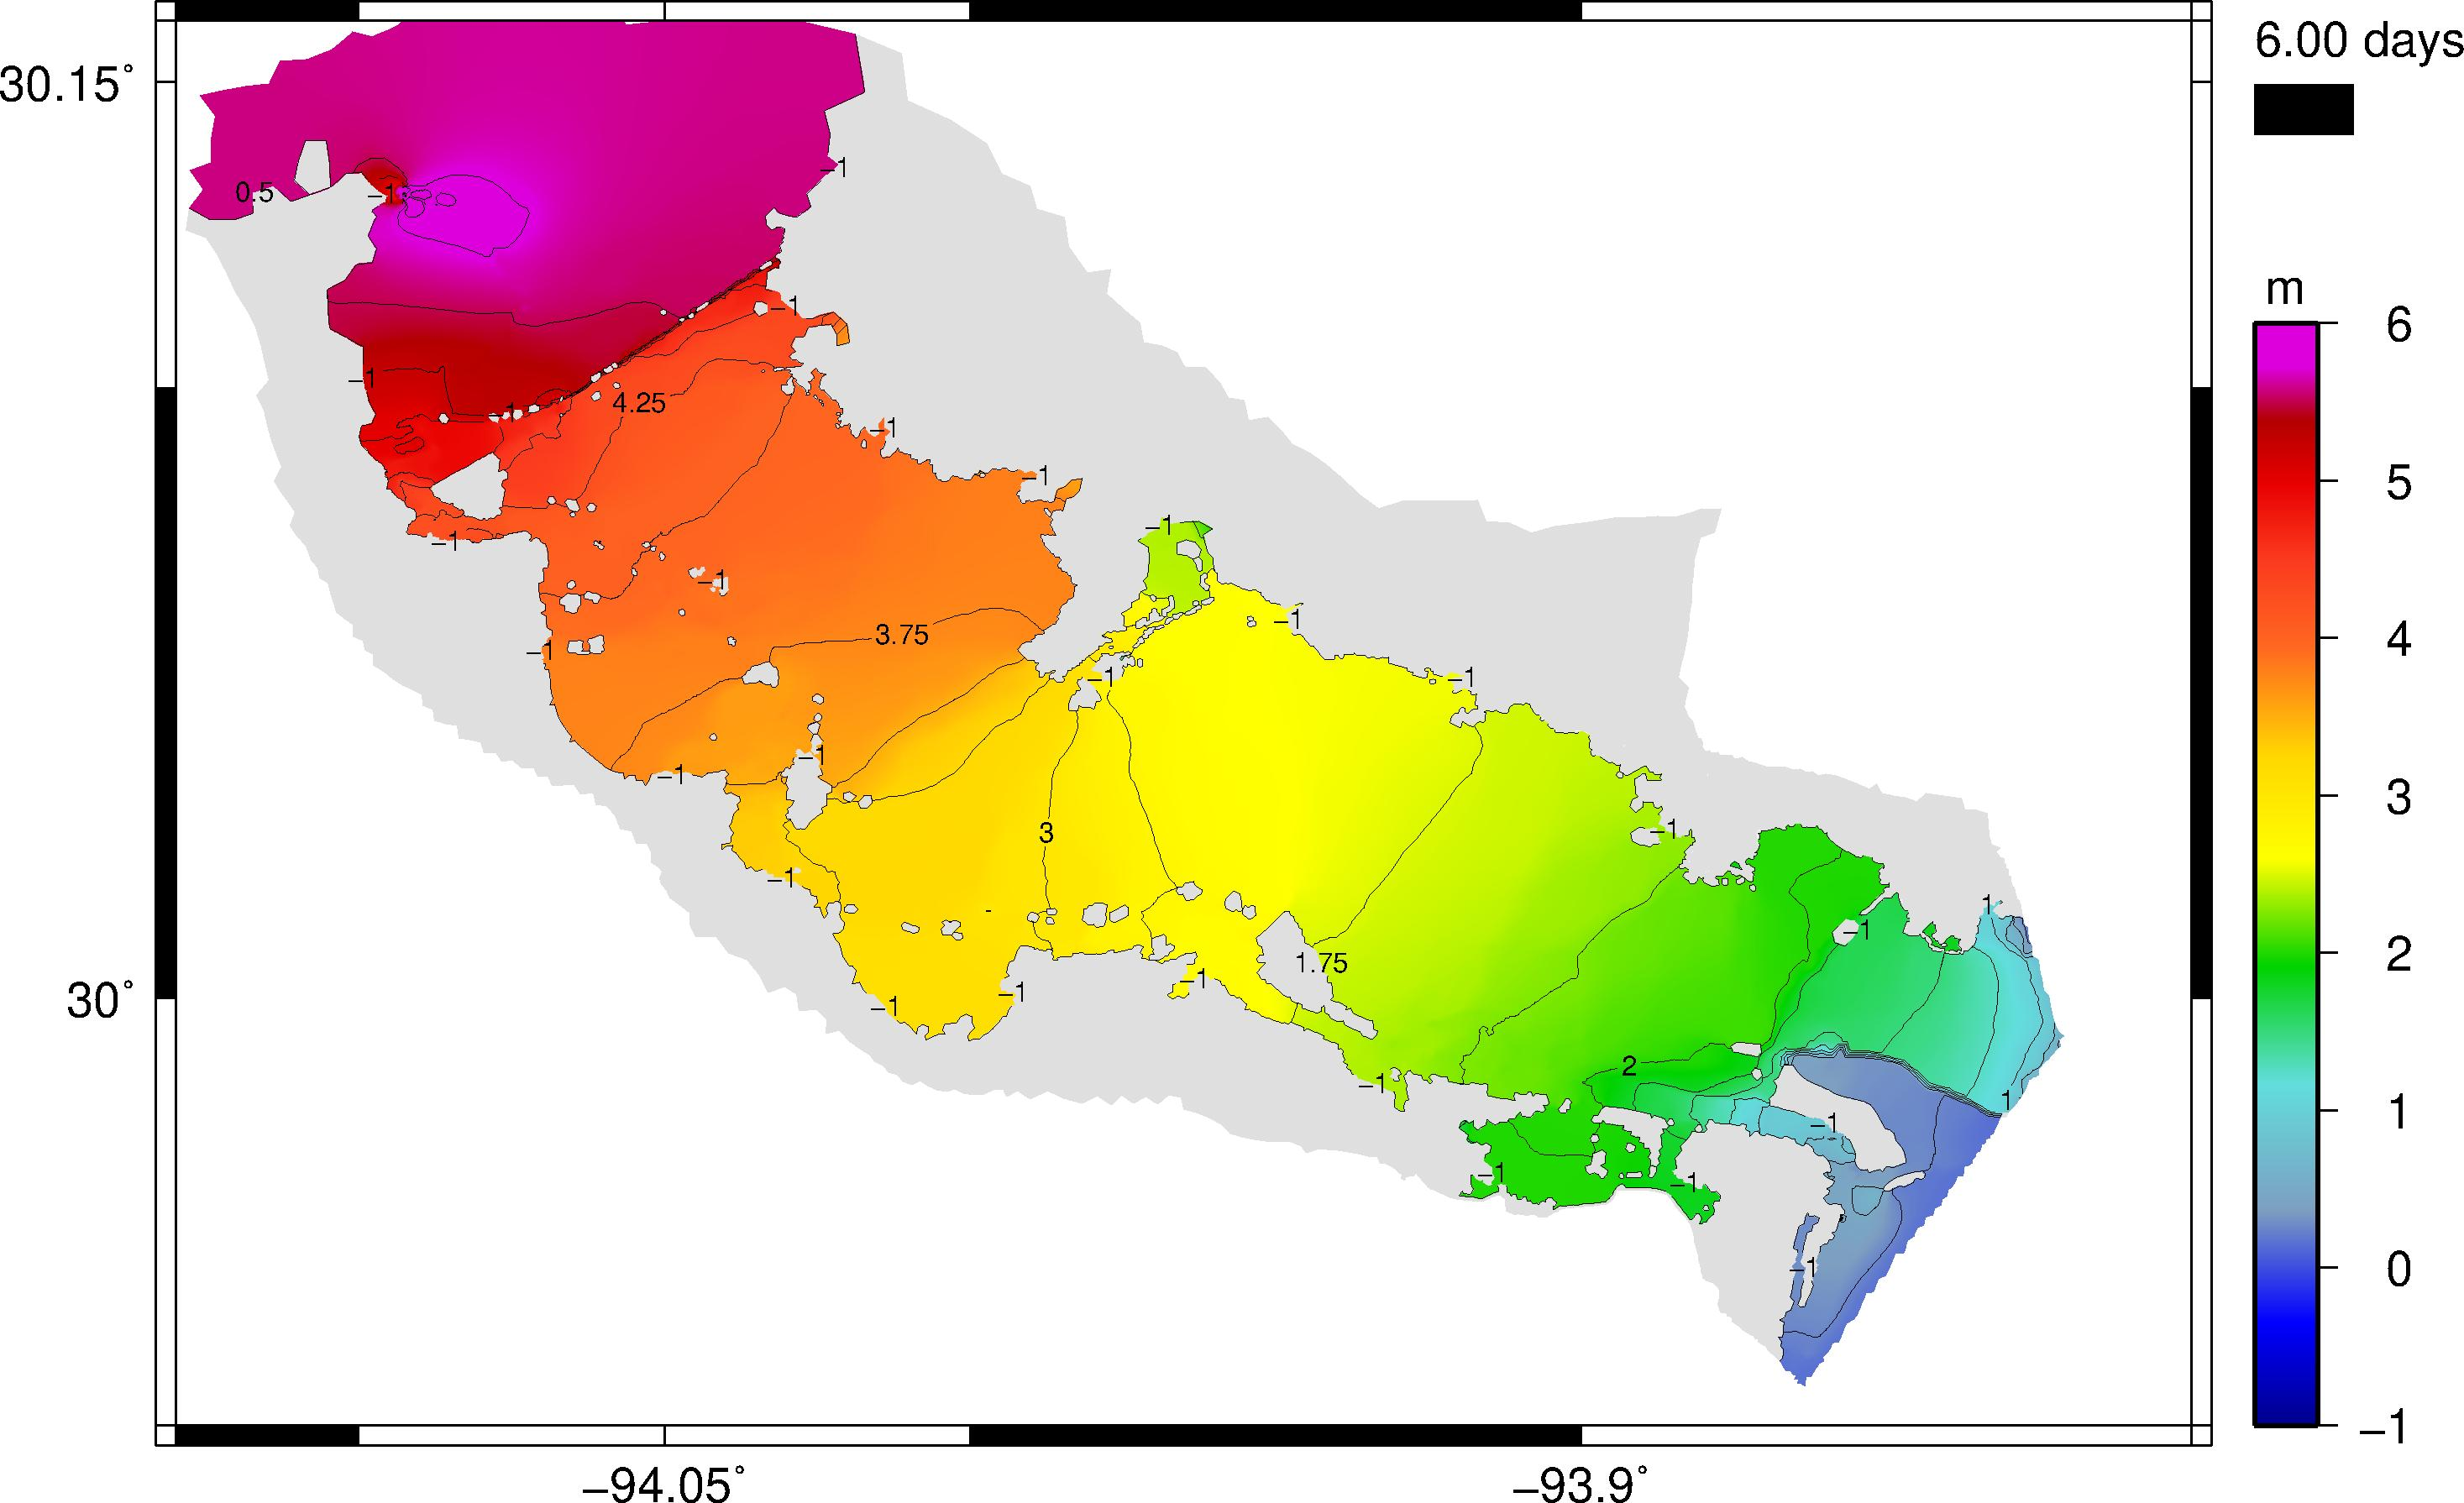
\includegraphics[width=0.95 \linewidth]{media/rain.jpg}
    Figure 3: Elevation plot of the Neches domain after 6 days. The river is inundated by river discharge from the top left as well as constant rainfall.
\end{center}

We also plot the elevation time series at two recording stations: Rainbow Bridge and Galveston Bay. As expected, when rain is added, the elevation is growing faster. The gauge data is also plotted.
\begin{center}
%\vspace{-1.0cm}
\begin{minipage}[h]{0.475\linewidth}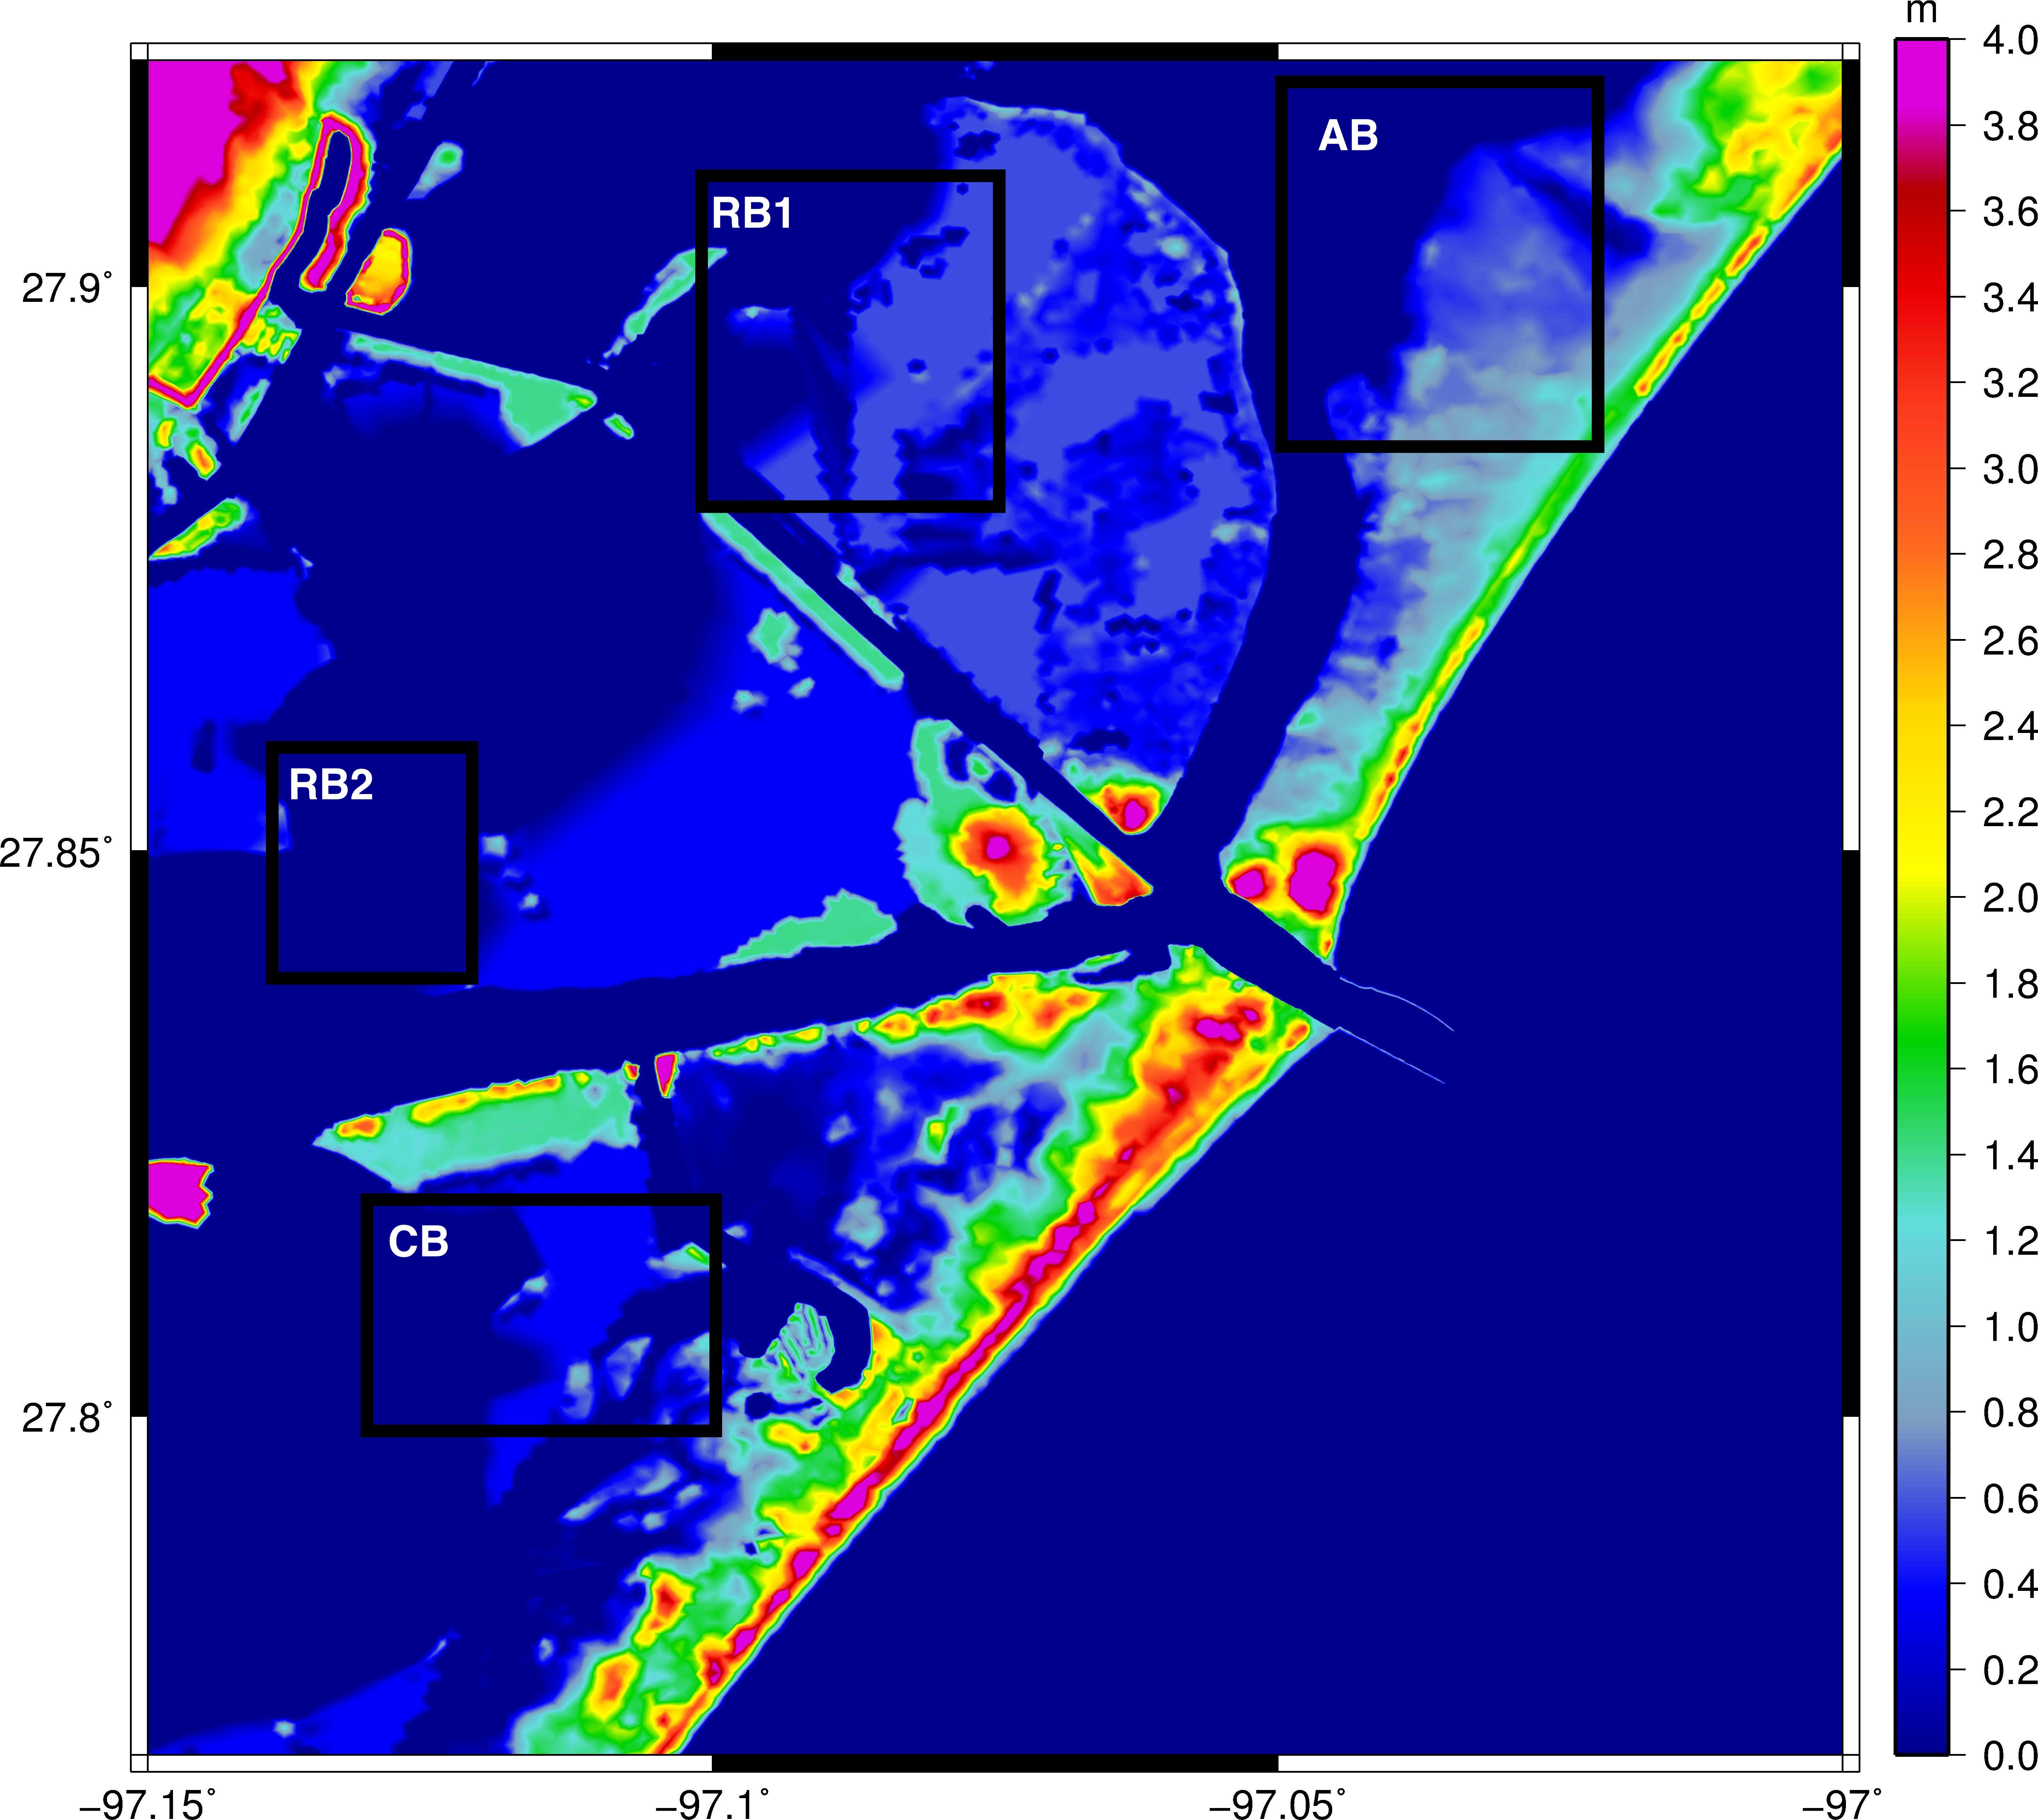
\includegraphics[width=1.0\textwidth]{media/images/Particle_tracking_highlight.jpg}\textbf{  Locations of Red drum larvae nursery grounds.}
\end{minipage}
\quad\begin{minipage}[h]{0.475\linewidth}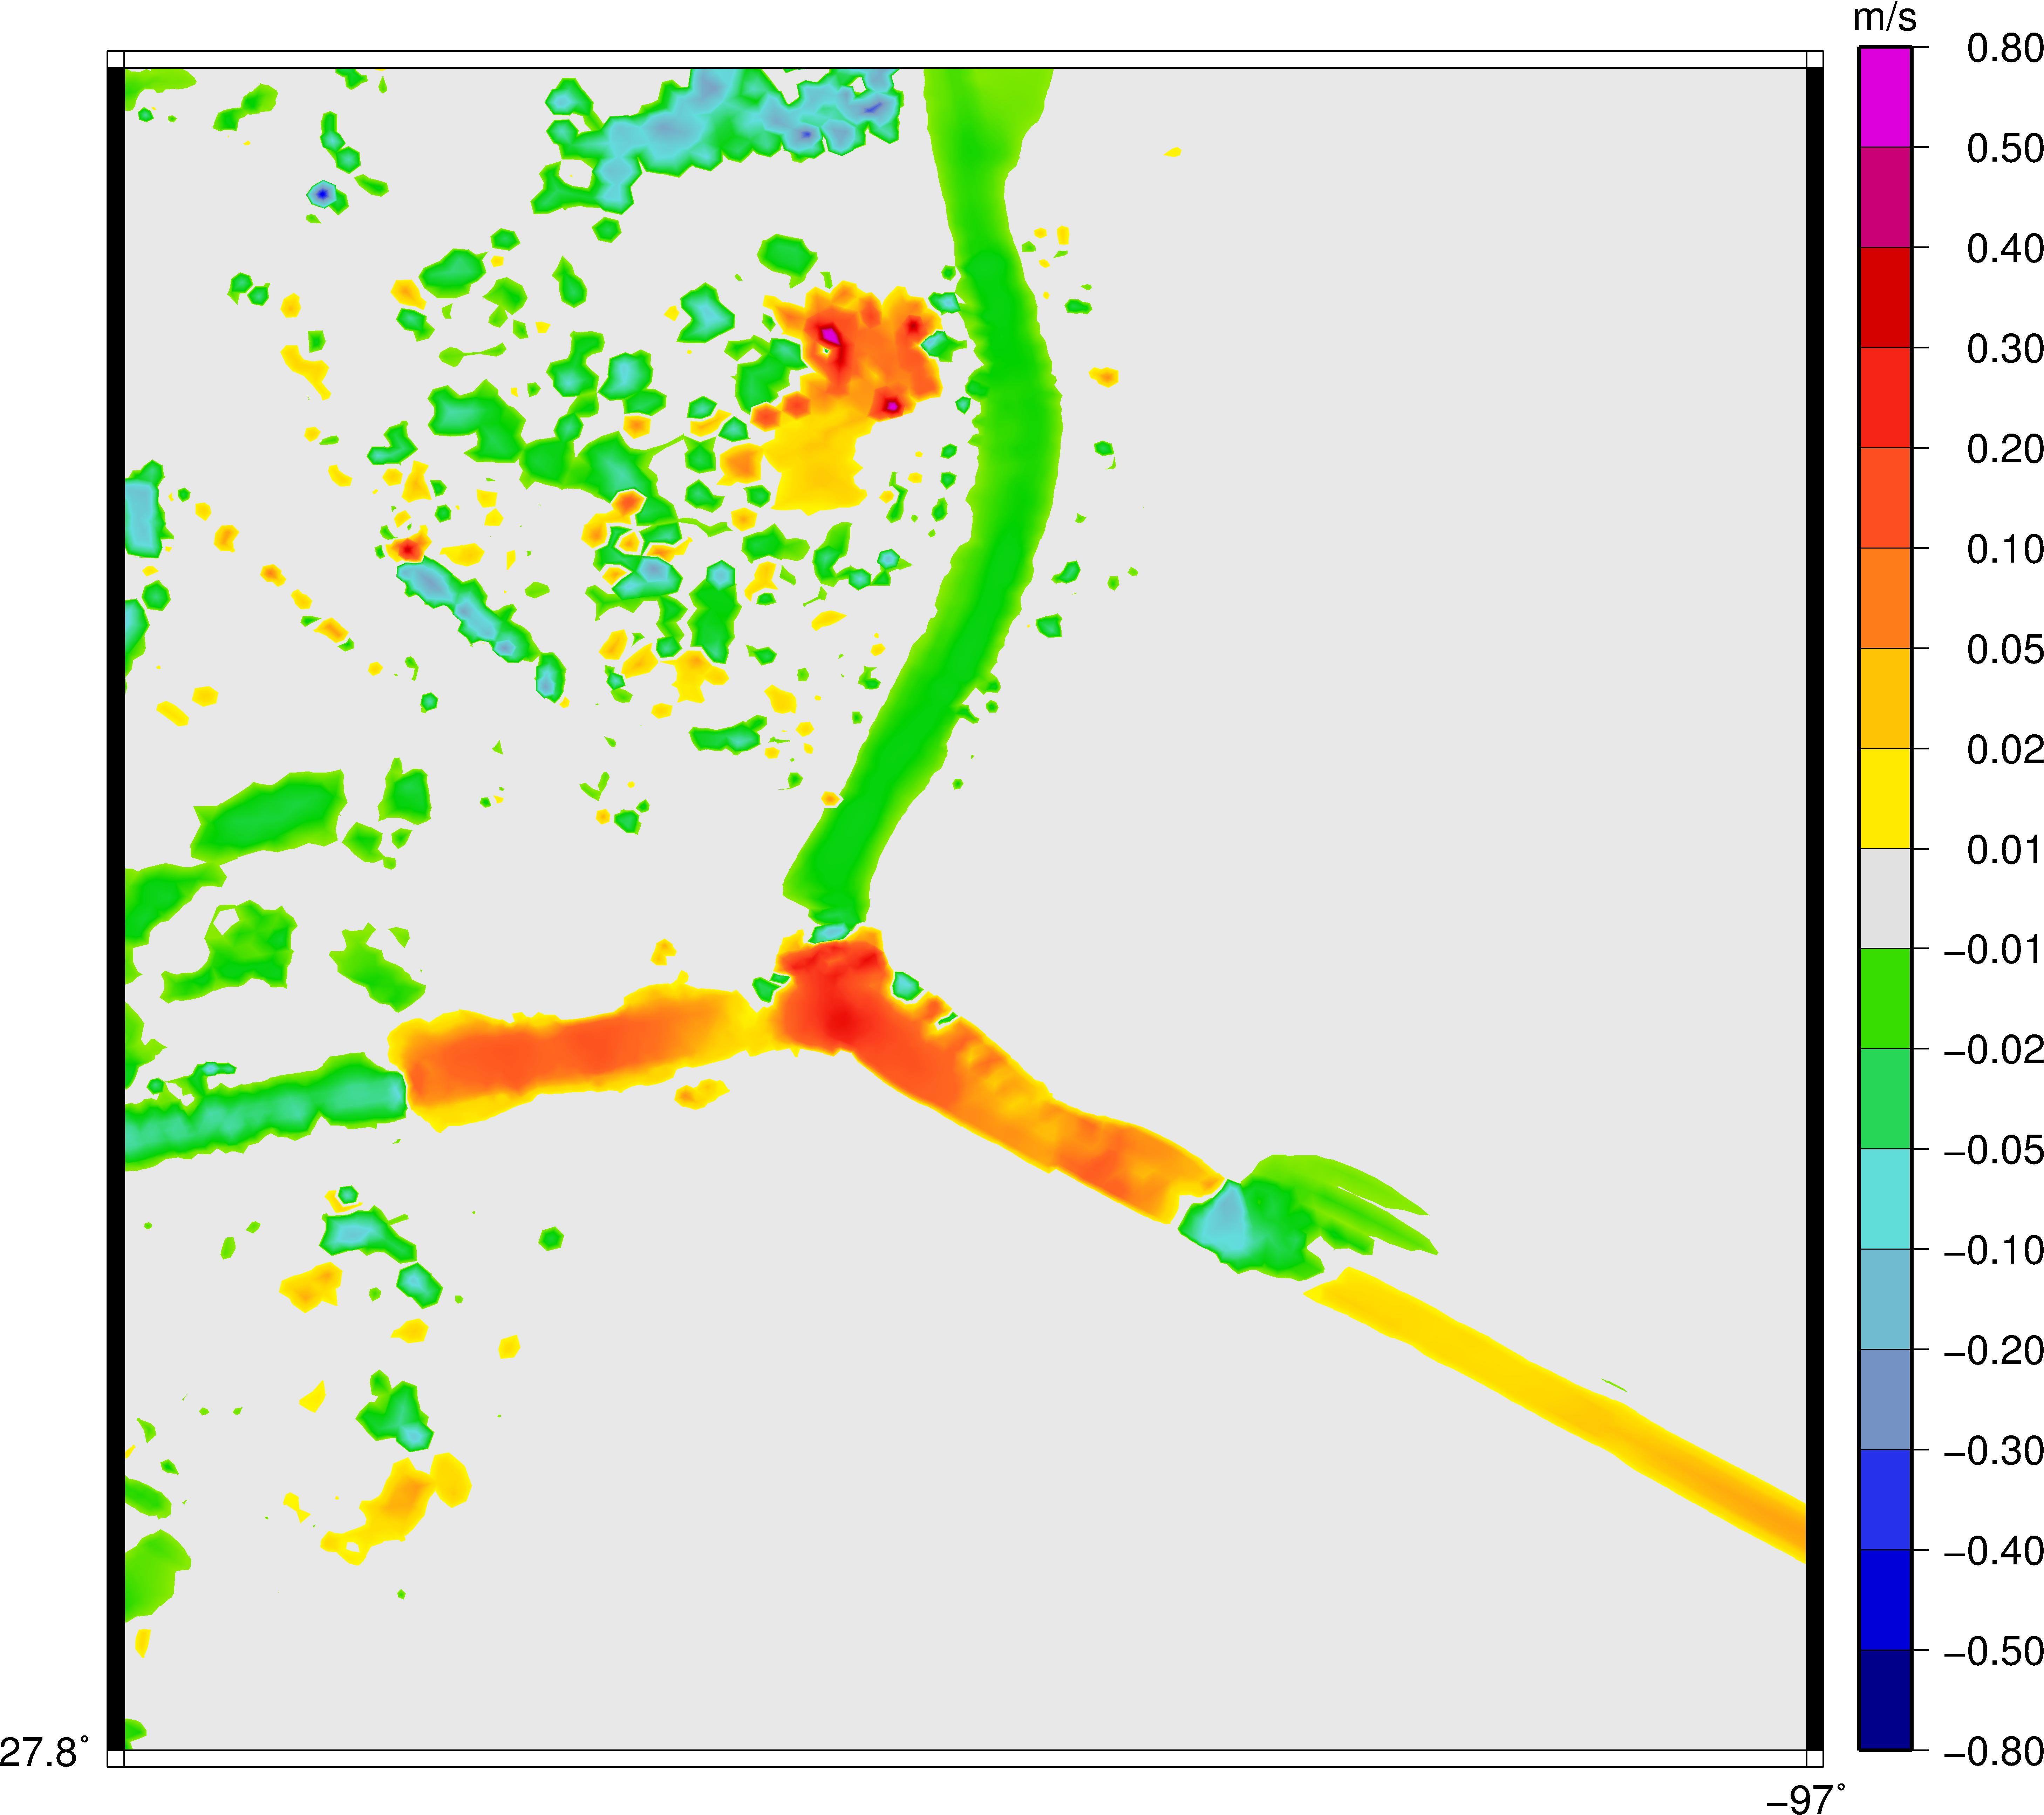
\includegraphics[width=1.0\textwidth]{media/images/velocity_comp_120001.jpg}\textbf{  Velocity Change in the Aransas Pass.}
\end{minipage}
%\caption{\label{fig:bathy}  bathymetry (in meter) near the Aransas Pass.}
\end{center}
%
%\vspace*{-0.7cm}
\section*{Proposed Work}
\noindent The number of larvae that ended up reaching the above bins was shown to be highly dependent on initial condition with the difference in success rates varying as much as 22 percent between any given initial configuration. The number of larvae reaching the grass beds also differed widely between the year with the drought, 2012, and the average year, 2019 with an average difference in success rate of 7$\%$ between years. However, at each given initial condition, the differences in success rates for the case with the current channel vs the deeper channel were low with an average increase of 1.0$\%$ in success rate across all cases for the deeper channel.


\renewcommand{\bibfont}{\fontsize{20}{20}\selectfont}
\nocite{*}
\printbibliography



\end{multicols}

\end{document}
